\documentclass[a4paper,11pt]{article}
\usepackage[T1]{fontenc}
\usepackage[utf8]{inputenc}
\usepackage{lmodern}
\usepackage[francais]{babel}
\usepackage[top=2.5cm, bottom=2.5cm, left=2.5cm, right=2.5cm]{geometry}

%image
\usepackage{graphicx}

\usepackage{array,multirow,makecell}
\setcellgapes{1pt}
\makegapedcells
\newcolumntype{C}[1]{>{\centering\arraybackslash }b{#1}}

\title{Approche sémantique de segmentation et de recherche interactive par le contenu issu d’une caméra de profondeur}
\author{Elliot Vanegue}

\begin{document}

\maketitle
\newpage

\section*{Remerciement}
\newpage

\begin{abstract}
\end{abstract}
\newpage

\tableofcontents
\newpage

%%%%%%%%%%%%%%%%%%%%%%%%%%%%%%%%%%%%%%%%%%%%%%%%%%%%%%%%%%%%%%%%%%%%%%%%%%%%%%%%%%%%%%%%%%%%%%%%%%%%%%%%%%%%%%%%%%%%%%%%%
\section{Introduction}
\subsection{Contexte}
Durant mon master IVI\footnote{Le master Image Vision Interaction est 
une spécialité du master informatique de l'université de Lille 1}, 
nous avons l'occasion de réaliser un stage de fin d'étude. J'ai choisi de réaliser ce stage
dans l'équipe 3D-SAM du laboratoire CRISTAL spécialisé dans l'acquisition et le traitement d'image 3D 
à partir de capteur 3D de type Microsoft Kinect. Leurs principaux travaux portent sur
l'analyse de forme d'objet 3D et la modélisation des variations des formes dans des
vidéos 3D. Réaliser mon stage dans un laboratoire était une priorité, car mes projets d'avenir
ne sont pas encore parfaitement planifiés et ce stage me permet de me décider sur l'environnement
de travail qui me convient le mieux. Durant mes deux derniers stages en IUT et en licence 3, j'ai pu
observer les atouts et les contraintes de chaque environnement, cependant le stage que j'ai effectué 
durant mon année en IUT relevé plus de l'ingénieurie que de la recherche. Durant ce stage de deuxième
année d'étude, je n'ai pas eu à effectuer un état de l'art, ni à tester des méthodes proposées par 
d'autres laboratoires de recherche.\\

Ces deux années de master nous ont beaucoup appris sur le traitement d'image et la reconnaissance de 
forme 2D. Ces sujets m'ont particulièrement intéressé et je souhaite, durant ce stage, approfondir ces
notions sur des types de données plus complexes comme sur des images 3D. C'est pourquoi je réalise mon
stage dans l'équipe 3D-SAM avec qui j'avais déjà travaillé sur mon projet de fin d'étude. Cette équipe
dirigée par M. Daoudi comprend cinq membres permanents, un post-doctorant et quatre doctorants. Mes 
encadrants durant ce stage sont M. Vandeborre et M. Wannous. Ce stage se déroule dans le cadre du
projet CrABEx qui concerne la production et l'édition de produits 3D pour des applications de
loisir. L'enjeu de ce projet est d'aider les designer 3D dans la création et l'édition de ressources
graphiques, en suggérant des éléments appropriés durant leur processus de création ou en générant automatiquement 
de nouvelles ressources à partir d'éléments existants.

\subsection{Objectif du stage}
Comme nous pouvons le constater depuis quelques années, les approches 3D intéractives sont de plus en plus 
présentes dans nos vies, que ce soit dans le domaine de la médecine avec l'utilisation de simulateur
pour apprendre à réaliser des opérations complexes, dans le loisir avec les jeux vidéo dont le revenu
mondial en 2015 est de plus de 90 milliards de dollars ou encore dans l'industrie pour visualiser des produits.
L'engouement pour cette technologie requiert des outils de plus en plus efficaces et rapides permettant à
des personnes de profession plutôt artistique de laisser place à leur imagination sans s'inquiéter de 
l'aspect technique.\\

Le fait de pourvoir modéliser dans un monde virtuel des objects du monde réel, et de pouvoir modifier ces 
objets facilement permettrait au designer de se soustraire de certaines tâches. On peut par exemple modéliser
une scène ou une personne facilement grâce à une caméra Kinect, puis effectuer des modifications sur le modèle résultant. Il serait
intéressant de récupérer le modèle 3D d'une personne et de modifier quelques unes des parties de son corps avec
des membres improbables comme un bras de robot. Le principe est le même dans une pièce, si nous souhaitons remplacer
des meubles d'une pièce intérieure par d'autres plus étonnants. L'intêret de cela est d'éviter à un designer de 
devoir remodéliser une personne ou une pièce existante qui serait déjà idéale pour ce que l'on souhaite réaliser.\\

Ce genre de technologie existe déjà pour modéliser des visages ou des gestes dans des jeux vidéo ou des films d'animation. 
Il y a par exemple des capteurs optiques basés sur des caméras infrarouges avec des marqueurs réfléchissants. La Kinect fait
également partie des outils de capture de mouvement, mais elle reste très peu utilisée dans le milieu professionnel.

\subsection{Problèmatique}
Les caméras 3D nous permettent d'obtenir un nuage de points de l'environnement qu'elles enregistrent. Cependant, ce 
type de caméra est peu précis et celles-ci sont souvent bruitées et comportent des valeurs qui n'existent pas dans le monde 
réel. 
%Ce bruit dépend de plusieurs facteurs comme la luminosité de l'environnement dans lequel nous effectuons l'acquisition,
%ou tout simplement la qualité et la précisions du capteur utilisé. 
La première difficulté lors de ce projet est de réussir à filtrer les données, de sorte qu'il ne reste que les données réellement présentes.
L'ensemble des données ne nous intéresse pas forcément. Nous devons donc passer par une phase de segmentation des données,
afin de détecter les objets présents dans une scène 3D.
En effet, si nous travaillons sur le corps humain, nous n'avons
pas besoin de l'environnement qu'il y a autour, ce surplus de données nous dérange lors de nos traitements. Il faut
donc trouver une solution permettant de segmenter les données que nous recevons, afin de ne garder que certains objets.\\ 
 
Une fois que les données ont été triées, nous avons besoin de reconnaitre les objets présents dans notre scène. Par exemple, dans
le cas du corps humain, si nous souhaitons modifier une partie du corps comme la main, il faut d'abord savoir quel partie du corps représente 
la main. La reconnaissance d'objet dépend fortement du type de données et nécessite généralement d'avoir une base d'apprentissage 
assez volumineuse. Lors de la modification d'une partie de la scène, il est nécessaire de connaître la position de l'objet remplacé, afin de pouvoir
placer le nouvel objet au même endroit et dans le même sens. Cette partie est très délicate surtout pour des membres humains, car
si le repositionnement n'est pas parfait et qu'il y a un écart entre deux membres, la scène perd toute sa crédibilité et son 
réalisme.\\

Les données que nous recupérons via la Kinect sont des données 2.5D. En effet, dans ce type de données nous récupérons des 
informations de profondeur, mais nous ne pouvons récupérer les informations occultées comme le dos de la personne qui est face à la caméra.
La solution que nous souhaitons mettre en place doit remplacer des données en 2.5D par des données 3D de synthèse. Nous devons donc
trouver une solution permettant de mettre en correspondance les caractèristiques de ces deux types de données.\\

Nous avons donc trois problèmatiques majeures dans ce projet : 
\begin{itemize}
  \item Comment filtrer les données de manière à ne traiter que celles qui nous intéressent ?
  \item Comment reconnaître automatiquement un objet dans une scène 3D ?
  \item Comment connaître la position et l'orientation exactes des objets présents dans notre scène ?
  \item Comment mettre en correspondance des informations 2.5D et 3D ?
\end{itemize}

\subsection{Organisation}

Pour répondre aux questions précédentes, j'ai travaillé sur deux applications mettant en avant des problématiques similaires,
mais avec deux façons différentes d'aborder ces problèmes. J'ai travaillé dans un premier temps sur une application qui se focalise
sur le corps humain. Cette application a pour but d'identifier les membres du corps, afin que l'utilisateur puisse les modifier
grâce à des modèles 3D existants. Les seules intéractions de l'utilisateur sont donc de cliquer sur le membre à modifier et de sélectionner
un modèle parmi ceux que l'application lui proposera afin de l'apparailler au reste du corps humain. 
La seconde application se concentre sur un environnement intérieur comportant plusieurs
objets. Ici le but est de segmenter la pièce pour reconnaître les objets présents afin de les ajouter dans une scène. Encore une fois,
l'utilisateur doit sélectionner un meuble et le modèle 3D qui lui convient dans une liste proposée par l'application.\\

Pour ce projet, j'utilise la caméra Microsoft Kinect v2, qui est l'une des caméras les plus utilisée dans la littérature. Le SDK fourni
avec cet outil comporte une segmentation du corps humain, la position du squelette de l'utilisateur et l'algorithme Kinect fusion qui
permet de construire un modèle 3D à partir du nuage de points fourni par la caméra.
Pour réaliser les deux applications, j'ai utilisé un ensemble de bibliothèques telles que la bibliothèque graphique de Microsoft pour
la réalisation de l'interface, la bibliothèque \og Point Cloud Librairie \fg\cite{PCL}(PCL) pour les calculs sur les nuages de points et 
opencv pour travailler sur les images couleurs et les images de profondeur fournies par la Kinect.\\

%TODO voir comment remplacer le " je vais" de la derniere phrase
J'ai dans un premier temps réalisé un état de l'art des solutions existantes sur les problèmatiques de segmentation et de reconnaissance de
forme à partir de nuage de points ou d'images de profondeur. Puis je vais décrire les solutions testées et appliquées aux deux applications que j'ai
développées durant ce projet.


%%%%%%%%%%%%%%%%%%%%%%%%%%%%%%%%%%%%%%%%%%%%%%%%%%%%%%%%%%%%%%%%%%%%%%%%%%%%%%%%%%%%%%%%%%%%%%%%%%%%%%%%%%%%%%%%%%%%%%%%%%
\section{Etat de l'art}
\subsection{Segmentation}
%recuperation d'un objet dans l'environnemnt -> interaction utilisateur
%dire que la création d'une base de connaissance est plus utile que pour le corps humain
La première étape lors de notre projet va être de segmenter les images que nous recevons de 
notre caméra. Les informations contenues dans une image 3D sont nombreuses et nous devons
déterminer les éléments important pour nos traitements. Dans notre scène,
nous avons besoin des objets proches ou du corps de la personne en face de la caméra, mais 
l'environnement autour des ces objets clés n'est pas important et doit être supprimer pour
gagner du temps lors de nos traitements en supprimant de l'information à traiter.
Une second segmentation est nécessaire pour le traitement du corps humain. Pour cette étape du projet,
nous devons segmenter le corps en plusieurs partie pour pouvoir par la suite les reconnaitres. Si cette
seconde segmentation n'est pas réalisé il ne nous sera pas possible de reconnaître les mains ou encore
la tête si nous ne savons délimité les parties du corps.  
 
\subsubsection{Scène intérieur}
De nombreux travaux ont été réalisé dans la segmentation d'image 2D avant que les caméras 3D ne soit
ouvert au grand public. Les premières méthode de segmentation reposaient sur la détection de contour
comme pour la méthode de P. Arbelaez et al\cite{2DSegmentation1}. Leur méthode repose sur le détecteur
de contour gPb qui est composé de d'un seuillage sur la luminance et sur la couleur et d'une détection
de texture. La fermeture des contours se fait ensuite en utilisant les superpixels. D'autres méthodes
2D utilise un simple seuillage en utilisant par exemple la méthode de N. Otsu\cite{Otsu} pour binariser
l'image et ainsi la segmenter.\\

%peut etre que l on peut rajouter des publi utilisant la depthmap
%voir si on sépare la depthmap et le nuage de point
Avec l'arrivé des caméras 3D de nombreuses recherche ont été effectué sur la segmentation d'image à partir
des information extraite de ce type de caméra. S.A.A Shah et al\cite{3DSegmentation1} utilisent les informations
de l'image de profondeur afin de calculer un vecteur sur chaque pixel. En applicant un seuillage sur la différence
des vecteurs ils obtiennent une segmentation de l'environnement qui leur permet de détecter des objets dans une pièce.
Il est possible à partir de l'image de profondeur de créer un nuage de point, ce qui permet d'obtenir les 
coordonnées 3D des points présents dans l'image de profondeur. Les informations qu'il est possible d'extraire
d'un nuage de point sont différentes et des méthodes de segmentation se sont développé autour de ces informations.\\

T. Rabbani et al\cite{pointCloudSegmentation} utilise les informations obtenus dans un nuage de point afin 
de calculer les normales de chaque point. Ils segmente ensuite l'image en comparant les normales et en appliquant
un seuillage sur cette comparaison. Si l'angle formé par les normales de deux points est super au seuil alors
les points appartiennent à deux régions différentes.

\subsubsection{Corps humain}
La segmentation du corps humain est un sujet très complexe, car contrairement au objet celui-ci bouge et adopte
des postures différentes. La méthode la plus souvent utilisé pour résoudre cette problématique est de déterminer
la posture de l'utilisateur et lorsque cette posture est connu il est facile de déterminer les différentes partie
du corps. Ces méthodes nécessitent d'avoir une base de connaissance contenant de nombreuses postures qui doivent
être segmenter et labelisé avec les différentes parties du corps. J. Shotton et al\cite{kinectSegmentation} ont
d'abord créé une base d'apprentissage en calculant un descripteur\footnote{Voir \ref{descriptor}}
et une technique d'apprentissage automatique appelé forêt d'arbres décisionnels\cite{randomDecisionForest}. 
Lorsque l'utilisateur bouge, le descripteur utilisé précédemment est recalculé sur l'image courante et le résultat 
est comparé au posture de la base d'apprentissage. La posture ayant une valeur proche du résultat calculé précédemment 
est la posture de l'utilisateur.

\subsection{Reconnaissance d'objets}
%FPFH
%SHOT
\subsubsection{Descripteur}
\label{descriptor}
\subsubsection{Apprentissave automatique}
%svm
%random forest
\subsubsection{Bag of word}

\subsection{Positionnement de modèle}
%moment d'inertie pour la position des membres
%PCA


%%%%%%%%%%%%%%%%%%%%%%%%%%%%%%%%%%%%%%%%%%%%%%%%%%%%%%%%%%%%%%%%%%%%%%%%%%%%%%%%%%%%%%%%%%%%%%%%%%%%%%%%%%%%%%%%%%%%%%%%%%%
\section{Modification des membres du corps humain}
\subsection{Etude de cas}
%on cherche a ne pas utiliser la kinect
Cette première application a plusieurs objectifs. Dans un premier temps, nous souhaitons réaliser 
une segmentation sans utiliser les outils fournis pas la Kinect, dans le but d'obtenir une méthode plus
précise ou, tout du moins, permettant d'améliorer une partie du procédé de segmentation. Comme nous l'avons vu dans 
l'état de l'art, les méthodes utilisées par la Kinect ont évolué et sont devenues plus stables et plus précises.
Le second objectif est de remplacer un nuage de points représentant un membre par un modèle 3D de ce même membre
mais ayant une forme différente. Cette première partie du stage me permet surtout d'aborder des concepts qui me 
serviront dans la seconde application qui est le but premier de ce stage.

\subsection{Délimitation du corps humain et minimisation de la quantité de donnée}
Durant cette première phase, nous travaillons sur un nuage de points et non sur les informations de l'image de profondeur.
Comme nous l'avons dit précédemment, l'ensemble des informations n'est pas pértinente pour les traitements que nous souhaitons
réaliser. La première étape dans la réalisation de cette application est de supprimer l'ensemble des informations qui ne se rapportent pas 
au corps humain. La première solution que nous développons consiste à utiliser deux seuils. Les points qui sont plus éloignés que le 
premier seuil, ainsi que les points en dessous du second seuil sont supprimés. 
Ces seuils sont les distances, en mètre, dans lequel l'utilisateur doit se trouver. Cette méthode est utilisée dans 
l'application ReconstructMe\footnote{\url{http://reconstructme.net}} qui est une application permettant de construire un modèle
3D complet à partir de données fournies par plusieurs images provenant d'une caméra 3D. Comme pour cette application, nous avons
décidé de laisser la possibilité à l'utilisateur de changer les seuils en fonction de son besoin.\\

\begin{figure}[!ht]
  \begin{center}
    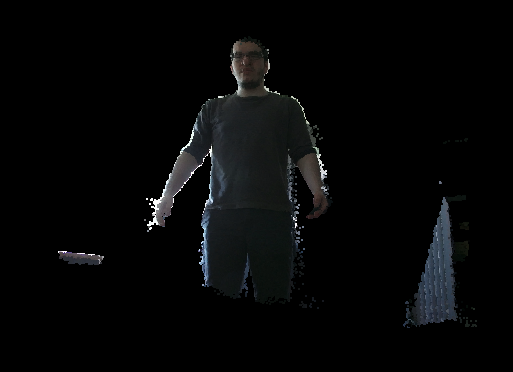
\includegraphics[width=8cm]{image/seuil1.PNG}
    \caption{Résultat d'une segmentation par seuillage}
    \label{fig:seuillage}
  \end{center}
\end{figure}

Nous pouvons voir sur la Fig. \ref{fig:seuillage} que le seuil permet effectivement de supprimer beaucoup d'informations
correspondant à l'environnement, mais qu'il reste beaucoup de bruit dû à la qualité de l'acquisition de la caméra ainsi que 
des objets qui se trouvent à la même distance que l'utilisateur. La librairie
PCL\cite{PCL} nous fournit beaucoup d'outils pour ce genre de problèmatique. Il y a une classe appelée \textit{StatisticalOutlierRemoval}
qui permet de supprimer les points supposés être du bruit. Pour cela, cette classe calcule la distance moyenne d'un point avec son
voisinage et si cette moyenne est trop élevée, elle supprime le point en question. Cependant, l'utilisation de cette classe ne
suffit pas à supprimer les objets à la même distance que l'utilisateur, car la densité de points de ces objets leur permet d'avoir
suffisamment de voisins proches pour avoir une moyenne de distances très petites. Pour pallier à ce problème, nous avons ajouté un
système de sélection permettant à l'utilisteur de sélectionner les données ne faisant pas partie du corps humain.\\

Pour la suite des traitements que nous souhaitons réaliser, il est préférable d'avoir un minimum d'informations et de ne garder
que ce qui est pertinent. Le corps humain que nous avons réussi à délimiter comporte encore beaucoup trop de données. Le nombre
de points fourni par la Kinect est très important et très concentré, il est possible de supprimer des points qui sont trop 
proches les uns des autres. Là encore PCL\cite{PCL} peut nous aider avec la classe \textit{VoxelGrid}. Cette classe crée une grille de
voxels sur le nuage de points, dont la taille est définie par l'utilisateur. L'ensemble des points, à l'intérieur d'un voxel, sont 
approximés en un point qui correspond au centroïde du voxel. Grâce à l'ensemble de ces traitements, nous ne gardons que l'information 
essentielle à nos traitements.

\subsection{Calcul de la distance géodésique}
Notre première idée pour segmenter le corps humain est d'utiliser la distance géodesique. Y. Liu et al\cite{GIF} montre que la distance
géodesique pour une même personne, quelque soit sa posture, est toujours la même pour les points de ses membres. Le seul problème 
est que plusieurs membres ont la même distance géodésique, on ne peut donc pas associer un membre directement à une distance.
Cependant, il est possible de seuiller le corps et de calculer des descripteurs, afin de déterminer quel nuage de points
correspond à quel membre.\\

Avant de calculer la distance géodésique du corps humain, nous avons besoin de créer un maillage sur le nuage de points. Pour cela,
j'ai repris le principe utilisé pour le descripteur FPFH\cite{FPFH} pour la sélection des voisins. Dans un premier temps, je calcule
la distance euclidienne de chacun des points du nuage de points avec tous les autres. Pour la création du voisinage, nous considérons non
seulement le nombre maximum de points à prendre en compte, mais aussi la distance maximum d'un point avec les autres. Nous avons eu
de nombreux problèmes lorsque nous n'avions pas mis la seconde condition, car lorsque la main de l'utilisateur était trop proche de sa 
jambe, certains points de la main avaient des voisins dans la jambe. Cette partie de l'algorithme est la plus délicate, car nous ne pourrons
pas avoir un aussi bon maillage que sur un modèle 3D et la distance géodésique repose sur la qualité de celui-ci. Pour l'améliorer, nous avons créé deux paramètres que l'utilisateur peut modifier. Le premier paramètre est le nombre de voisins d'un point et
le second est la distance euclidienne maximale entre les voisins.\\

%TODO voir si on met des exemples de maillage defectueux 

A cette étape de l'algorithme, nous avons donc un maillage et les distances euclidiennes de chaque point avec son voisinnage. Pour calculer
la distance géodésique du centroïde du nuage de points avec chaque point, nous allons utiliser l'algorithme de Dijkstra\cite{dijkstra}.
Il faut donc trouver le plus court chemin du centroïde jusqu'au point dont on veut calculer la distance géodésique, en passant par le
maillage que nous avons construit précédemment. Les valeurs prises en compte entre chaque point dans l'algorithme de Dijkstra seront
les distances euclidiennes entre les points. A chaque fois qu'un point est ajouté au chemin emprunté par l'algorithme il faut 
additionner la distance euclidienne entre ce point et le précédent, pour obtenir un résultat final correspondant à la distance 
géodésique entre le centroïde et le point dont on cherche la distance.\\

\begin{figure}[!ht]
  \begin{center}
    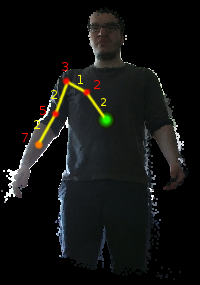
\includegraphics[width=5cm]{image/cheminGeodesique.PNG}
    \caption{Exemple de chemin parcouru par l'algorithme de calcul de la distance géodésique pour un point.
    Le point vert correspond au centre de gravité du corps, les points rouges sont les noeuds du chemin et le point 
    orange est le point d'arrivée. Les chiffres jaunes sont les distances pour aller d'un noeud à l'autre, et les chiffres
    rouges sont la distance géodésique au noeud correspondant.}
    \label{fig:cheminGeodesique}
  \end{center}
\end{figure}

\begin{figure}[!ht]
  \begin{center}
    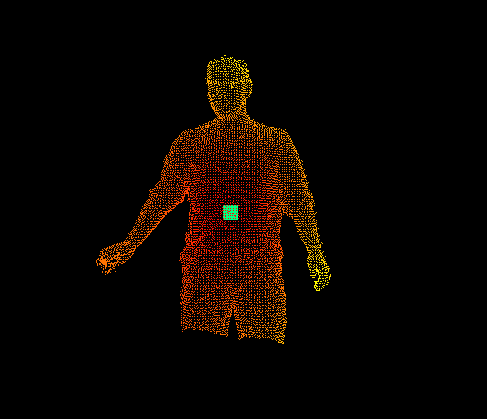
\includegraphics[width=6.5cm]{image/geodesic1.PNG}
    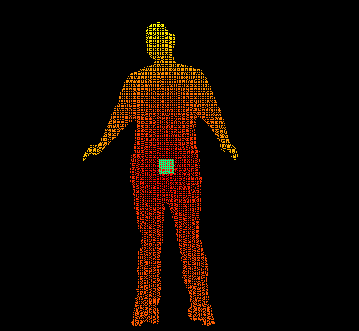
\includegraphics[width=6cm]{image/geodesic2.PNG}
    \caption{Résultat du calcul de la distance géodésique sur l'ensemble du nuage de points. Le point vert correspond au centroïde du
    nuage de points. Plus la couleur des points est proche du rouge, plus les points sont proches du centroïde.}
    \label{fig:geodesique}
  \end{center}
\end{figure}

Sur les images de la Fig. \ref{fig:geodesique}, on peut voir que la distance géodésique n'est pas aussi précise qu'on le souhaiterait.
Dans la première image, on voit que la distance géodésique n'est pas la même sur le bras gauche et sur le bras droit. Cette imprécision
vient de la qualité du maillage. Certains points ne passent pas par le corps et traversent dans le vide du ventre au bras, ce qui réduit
la distance géodésique au niveau des mains. Dans la seconde image, on voit que la position du centroïde est très importante. Celle-ci change en fonction de ce que l'on voit du corps humain, ce qui modifie également la distance géodésique. Un simple seuillage
n'est donc pas suffisant pour segmenter le corps humain, car de trop nombreux paramètres interviennent dans le calcul de la distance géodésique,
y compris la physionomie de l'utilisateur.

\subsection{Segmentation du corps humain}
%recherche du point le plus éloigné puis suppression d'un groupe de point ....
%voir si on parle des superpixels
Malgré un léger manque de précision de la part du calcul de la distance géodésique sur le corps humain, nous avons testé une
méthode de segmentation qui ne prend pas en compte cette imprécision. Le principe de cette segmentation est de détecter le
membre le plus éloigné, puis de le supprimer dans la recherche des autres membres. Pour cela, notre algorithme recherche le point
dont la distance géodésique est la plus grande et forme une zone autour de ce point. Cette zone a un rayon prédéfini qui sera le 
même pour chaque membre. Les points à l'intérieur de cette zone seront enregistrés et sont considérés comme faisant partie d'un 
même membre. Ils seront ensuite supprimés du nuage de points du corps humain, afin de ne pas être pris en compte dans les 
étapes suivantes.\\

\begin{figure}[!ht]
  \begin{center}
    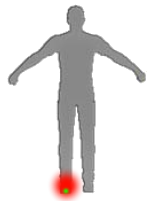
\includegraphics[width=3cm]{image/humanFootR.png}
    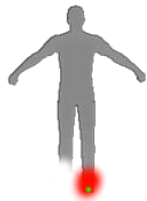
\includegraphics[width=3cm]{image/humanFootL.png}
    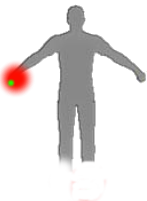
\includegraphics[width=3cm]{image/humanHandR.png}
    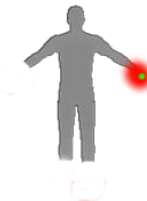
\includegraphics[width=3cm]{image/humanHandL.png}
    \caption{Premières étapes de l'algorithme de segmentation du corps humain. Le point vert correspond au point le plus éloigné et la zone rouge correspond à
    l'ensemble des points considérés comme faisant partie du membre.}
    \label{fig:segmentation}
  \end{center}
\end{figure}

Y. Liu et al\cite{GIF} proposent une amélioration de leur méthode basée sur le superpixel SLIC\cite{SLIC}. Le but de l'utilisation du superpixel
SLIC est de diminuer le nombre de points pris en compte lors des calculs du plus court chemin de l'algorithme de Dijkstra afin de diminuer le 
temps de calcul. Cela permet également d'améliorer la segmentation du corps humain. Le seul paramètre de l'algorithme SLIC est le nombre de classe à 
retrouver dans l'image. Cet algorithme s'effectue en général dans l'espace colorimètrique LAB. La méthode de Y. Liu et al\cite{GIF} quant à
elle, utilise les coordonnées x, y et z. Après avoir testé l'utilisation des superpixels, nous remarquons que nous obtenons plus rapidement le résultat,
mais que celui-ci n'est pas meilleur que celui que nous obtenions précédemment.\\

%TODO mettre une image avec les superpixel en rouge
%TODO faire une comparaison entre les résultats obtenu avec et sans les superpixel

Cette méthode est efficace pour reconnaitre les extrémités du corps humain comme les mains, les pieds et la tête. Le reste des parties du corps 
est moins précis, notamment au niveau des épaules où le point de la zone est très instable et peut se retrouver au niveau du torse. De plus, la taille 
des zones dépend de la physionomie de la personne devant la Kinect. 

\subsection{SDK de la Kinect}
Etant donné que nos résultats pour la segmentation du corps ne sont pas suffisamment précis pour la suite de nos traitements et par faute de
temps, nous avons décidé d'utiliser les outils fournis avec la Kinect pour continuer le projet. Grâce à la caméra de Microsoft, nous pouvons
récupérer le squelette de l'utilisateur dont les articulations sont labellisées avec le nom de la partie du corps humain à laquelle elle appartient
(voir Fig. \ref{fig:kinect}.a). De plus, la Kinect nous permet de séparer les points qui appartiennent à l'utilisateur de ceux qui appartiennent
à l'environnement (voir Fig. \ref{fig:kinect}.b).\\

\begin{figure}[!ht]
  \begin{center}
    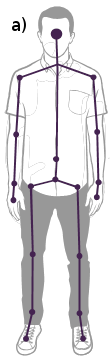
\includegraphics[width=2cm]{image/kinectSkeleton.png} 
    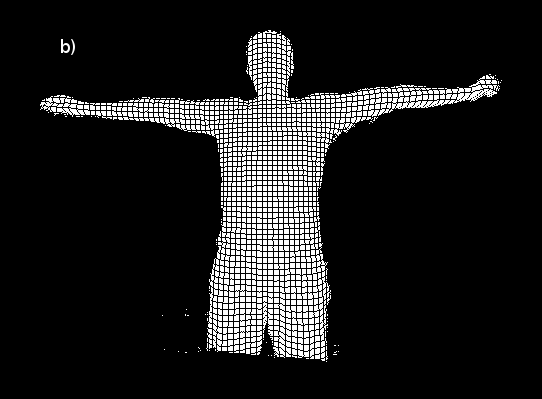
\includegraphics[width=8cm]{image/seg1.PNG}
    \caption[The LOF caption]{a) Squelette fourni par la caméra Kinect\footnotemark et b) séparation du corps humain de l'environnement}
    \label{fig:kinect}
  \end{center}
\end{figure}
\footnotetext{source : \url{http://hdimagelib.com/standing+person+sideways?image=356490844}}

Grâce à ce squelette et au nuage de points, nous pouvons segmenter le corps humain. Pour cela, pour chaque articulation nous définissons une zone
dont la taille est variable en fonction de l'articulation. Les points du nuage sont labellisés en fonction de leur distance avec les articulations.
Donc, un point prend le label de l'articulation dont il est le plus proche.\\

\begin{figure}[!ht]
  \begin{center}
    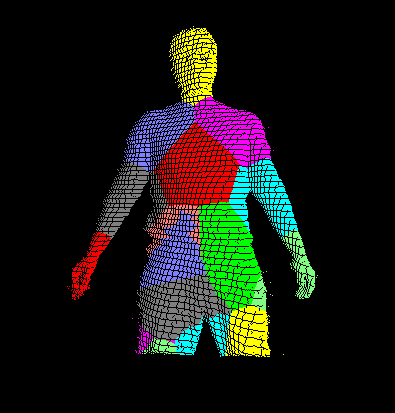
\includegraphics[height=4cm]{image/lab1.PNG} 
    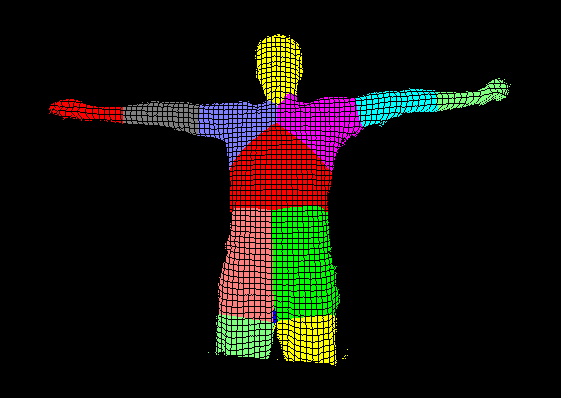
\includegraphics[height=4cm]{image/lab2.PNG}
    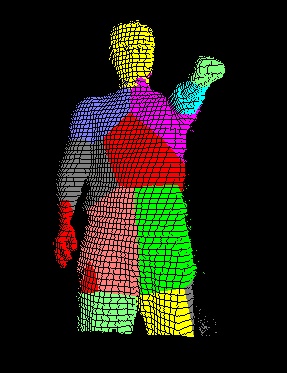
\includegraphics[height=4cm]{image/lab3.PNG}
    \caption{Résultat obtenu avec la segmentation du corps humain via les outils de la Kinect}
  \end{center}
\end{figure}

Nous pouvons voir que comme nous l'attendions, le résultat de cette segmentation est bien meilleur puisque nous avons à notre disposition
beaucoup plus d'informations qu'auparavant grâce au squelette de l'utilisateur. Même si cette segmentation n'est pas parfaite, comme on peut
le voir dans la première image, elle reste suffisante pour nos futurs traitements. En plus de la segmentation, nous connaissons déjà le nom
des membres grâce aux labels des articulations. Nous n'avons donc pas besoin de passer par une étape de reconnaissance des parties du
corps, car celle-ci a déjà été réalisée par les outils de la Kinect. Il ne reste plus qu'à supprimer le bruit présent dans les membres, les points
mal labelisés, grâce à la classe StatisticalOutlierRemoval que nous avons vu précédemment.

\subsection{Positionnement}
La dernière étape de cette première application est d'échanger le nuage de points d'un membre du corps par un modèle 3D représentant cette même partie
du corps. Cette étape est très complexe à cause de deux problèmes majeurs. Tout d'abord, le type d'information n'est pas le même. Dans un cas, nous avons
un nuage de points dont les points sont très concentrés, mais avec des parties occultées. De l'autre côté, nous avons un modèle 3D avec un nombre de points
inconnus, donc une concentration de points inconnu, mais sans zone occultée si nous prenons en considération le maillage du modèle. Le second problème
est que le but recherché est de remplacer la partie du corps humain par quelque chose de plus improbable et étonnant comme une partie du corps d'un monstre,
d'un robot ou d'un corps dont la musculature est différente.\\

Nous testons dans un premier temps l'algorithme le plus utilisé dans la littérature en terme de correspondance de modéle 3D. L'algorithme ICP\cite{ICP} est
disponible dans la librairie PCL\cite{PCL}. Après plusieurs tests sur différentes parties du corps, nous pouvons voir que l'algorithme ICP arrive à déterminer
la bonne translation, si on compare les centroïdes des modèle 3D avec leur partie du corps correspondant. Cependant, ICP ne parvient pas à déterminer
l'orientation du modèle. Le problème vient du fait que les données ne sont pas les mêmes. Bien que celles-ci soient différentes, la forme générale
d'une partie du corps reste la même, que ce soit un modèle ou un nuage de points, donc sa boîte englobante reste similaire également. Nous utilisons la méthode
de moment d'inertie de S. Ushakov disponible dans PCL pour déterminer l'orientation du nuage de points à partir de la matrice de covariance
(voir Fig. \ref{tab:modelMatching}).\\

\begin{figure}[!ht]
  \begin{center}
    \begin{tabular}{C{2cm}|c|c}
      modèle & position 1 & position 2 \\
      \hline
      pince de crabe (main gauche) & 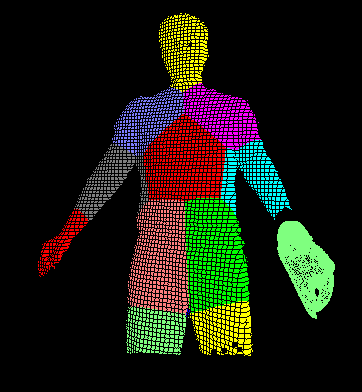
\includegraphics[height=4cm]{image/crabPlier1.PNG} & 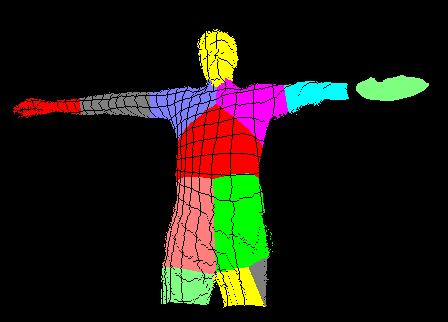
\includegraphics[height=4cm]{image/crabPlier2.PNG} \\
      \hline
      main robot (main gauche) & 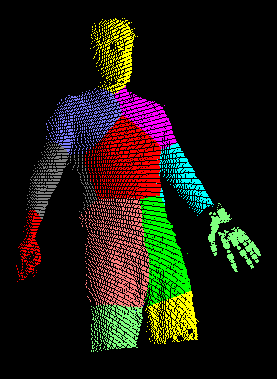
\includegraphics[height=4cm]{image/cyberHand1.PNG} & 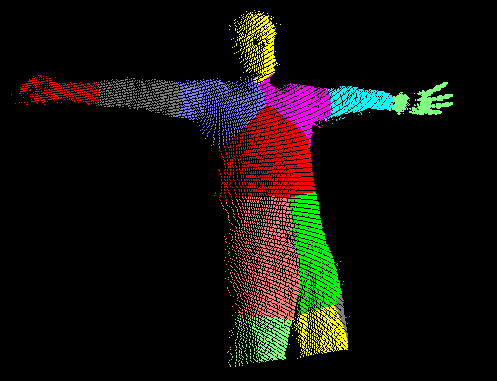
\includegraphics[height=4cm]{image/cyberHand2.PNG} \\
      \hline
      main cybord (main droite) & 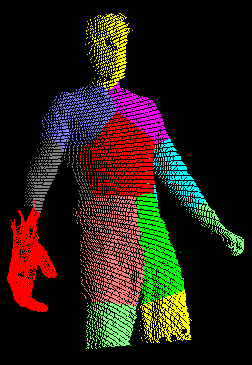
\includegraphics[height=4cm]{image/cyborgHand1.PNG} & 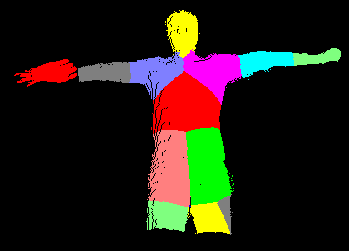
\includegraphics[height=4cm]{image/cyborgHand2.PNG} \\
      \hline
      main de monstre (main droite) & 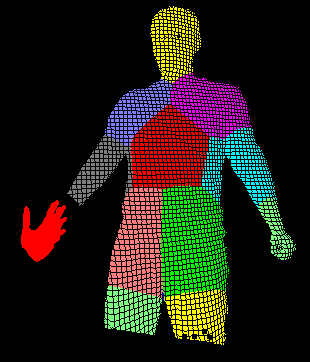
\includegraphics[height=4cm]{image/monsterHand1.PNG} & 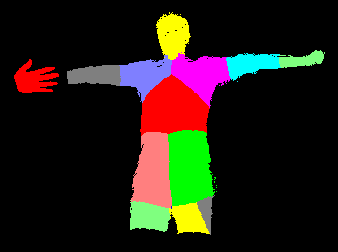
\includegraphics[height=4cm]{image/monsterHand2.PNG} \\
      \hline
      tête cyborg & 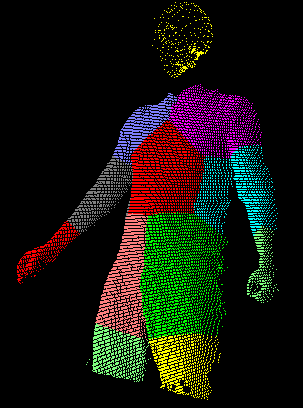
\includegraphics[height=4cm]{image/cyborgHead.PNG} &  \\
      \hline
    \end{tabular}
    \caption{Résultat de remplacement de parties du corps par des modèles 3D}
    \label{tab:modelMatching}
  \end{center}
\end{figure}

Nous pouvons voir sur les résultats de la correspondance de modéle, qu'il y a deux problèmes importants. Le premier problème est celui de l'orientation
de certains modèles 3D. Dans la majorité des tests que nous avons effectué, il y a au moins deux axes sur lequels l'orientation est la bonne. La méthode 
permet de déterminer l'orientation, mais pas le sens, ce qui implique que dans certains cas, l'un des axes soit visuellement tourné du mauvais côté.
Le second problème provient du non raccord du modèle avec le reste du nuage de points, qui est très bien illustré dans l'exemple de la pince de crabe.
Pourtant dans chacun des cas, la translation est juste. Nous le vérifions en comparant la position du centroïde entre le modèle 3D et le nuage de points
(il existe juste un petit décalage sur la profondeur à cause des zones occultées dans le nuage de points). Ce décalage est dû à une différence de ce qui est 
pris en compte comme étant une main (dans les exemples que nous avons vu). Dans le nuage de points, la zone considérée comme étant la main comporte la main et le poignet, alors que 
dans le modèle 3D de la main de monstre le poignet n'est pas présent.\\

Notre méthode serait suffisamment efficace pour remplacer deux nuages de points de membre du corps provenant d'une caméra 3D. On pourrait facilement
remplacer la tête de deux personnes.
Mais la mise en place d'une correspondance entre un nuage de points et un modèle 3D d'une partie du corps n'est pas suffisamment précise. Pour pallier
aux erreurs de l'application, nous avons envisagé de laisser la possibilité à l'utilisateur d'intéragir avec celle-ci. Le plus important est l'orientation
du modèle, et nous savons qu'en cas d'erreur, il faut effectuer une rotation du modèle de 180\degre sur l'un des trois axes. L'utilisateur devrait juste
sélectionner l'axe qui ne convient pas et l'application effectuerait la rotation seule. Maintenant que nous avons vu un cas particulier, nous allons pouvoir
partir sur une application plus généraliste et plus simple en réutilisant ce qui a été vu pour l'application sur le corps humain.  

\subsection{Travaux futurs et applications}
L'application que nous avons développée est vraiment la base, et de nombreuses extensions peuvent être ajoutées.
L'une d'entre elles est la possibilité de bouger la partie du corps modifié en temps réel. Pour l'instant, nous filmons
la scène et l'utilisateur doit mettre en pause l'acquisition lorsqu'il souhaite modifier une partie du corps. Lorsque le
processus est terminé, il serait intéressant de laisser la possibilité à l'utilisateur de relancer l'acquisition afin de
voir la nouvelle partie du corps se déplacer. La possibilité de changer des parties du corps en temps réel durant 
l'acquisition, serait un véritable plus, mais la difficulté à optimiser les calculs serait trop importante. Sur l'application
actuelle, nous sommes à 5 à 10s de calcul pour le remplacement d'une partie du corps.\\

Nous n'avons pas non plus eu le temps de développer l'interface de l'application. Pour l'instant, les modèles de remplacement
sont prédéfinis pour chaque membre, donc l'utilisateur ne peut pas sélectionner le modèle qu'il souhaite.\\

L'un des aspects sur lequel nous avons réfléchi était la construction d'un modèle complet, sans partie occultée, du corps
humain. Cette étape est réalisable avec un algorithme fourni dans le SDK de la Kinect qui est le \og kinect fusion \fg\cite{
KinectFusion}. Actuellement, nous mélangeons un nuage de points fourni par la Kinect, avec le dos de la personne occulté, et 
des modèles 3D dont on ne prend que les points. Même si le tout reste visuellement cohérent, on peut voir la différence entre
le nuage de points et le modèle 3D.
Cette extension permettrait, en plus d'une simple visualisation de l'utilisateur avec une partie du corps
différente, de reconstruire un maillage complet avec le corps de l'utilisateur. Ce nouveau modèle 3D pourrait alors être
directement utilisé dans un film d'animation ou un jeu vidéo.


%%%%%%%%%%%%%%%%%%%%%%%%%%%%%%%%%%%%%%%%%%%%%%%%%%%%%%%%%%%%%%%%%%%%%%%%%%%%%%%%%%%%%%%%%%%%%%%%%%%%%%%%%%%%%%%%%%%%%%%%%%%
\section{Reconstruction d'un environnement intérieur}
%\subsection{Segmentation de l'environnement intérieur}
%segmentation par l'utilisateur
%\subsection{Création d'une base de connaissance}
%utilisation opencv
%creation du dictionnaire
%calcul du descripteur des objets -> detail sur le nombre d'objet et sur le nombre d'exemplaire
%test sur une base composé de mesh et sur une autre composé de nuage de point
%\subsection{Reconnaissance des objets} 
%simple comparaison avec le descripteur
%TODO voir ce qu'on peut mettre dans cette section

\subsection{Objectif}
%interface
Le but de cette seconde application est de pouvoir modifier un environnement intérieur au travers d'une interface
simple et intuitive. 
Pour cela, nous allons dans un premier temps récupérer un nuage de points d'une pièce intérieure. Puis à partir
de ce nuage de points, nous allons segmenter la pièce afin de pouvoir détecter des objets à l'intérieur de celle-ci.
L'utilisateur doit ensuite sélectionner un objet, ce qui déclenchera l'apparition d'une liste contenant un ensemble de modèle 3D
d'objets équivalents à celui sélectionné. L'utilisateur n'a plus qu'à choisir l'objet qui lui convient dans la liste,
afin de l'ajouter dans un autre environnement 3D présent dans l'application.\\

Lors de ce scénario, nous pouvons voir qu'il y a deux grandes étapes qu'il faudra réaliser dans l'application. Tout d'abord, il faut 
segmenter le nuage de points de la pièce, dans le but de détecter des objets. Puis il faut reconnaître les objets détectés afin
d'afficher la bonne liste d'objets 3D. Nous avons décidé, pour faciliter le développement, de laisser l'utilisateur sélectionner
l'objet qu'il souhaite dans le nuage de points, afin de ne pas avoir à développer la détection d'objet dans le nuage de points.
Pour cela, nous nous inspirons des travaux de T. Shao et al\cite{interactiveSeg} et de J. Xiao et al\cite{interactionSeg2}.
Il nous reste donc à reconnaitre l'objet sélectionné par l'utilisateur.

\subsection{Création de la base d'apprentissage}
Afin de pouvoir reconnaître un objet, nous avons besoin d'un base d'apprentissage contenant les descripteurs d'un ensemble
d'objets. Pour créer cette base, nous utilisons la représentation du \og bag of word \fg ainsi que la méthode d'apprentissage 
automatique SVM\cite{SVM} disponible dans la librairie opencv. Pour la création de notre base, nous utilisons une vingtaine
d'images de six objets différents. Les nuages de points dont nous nous sommes servis pour la création de notre base viennent de 
K. Lai et al\cite{Base1} issue de M. Firman\cite{generalBase} qui a regroupé un ensemble de bases d'objets provenant de caméra 3D.\\

Le descripteur que nous utilisons pour cette application est le descripteur FPFH\cite{FPFH} qui est l'un des plus efficaces dans la
reconnaissance d'objet à partir de nuage de points. Nous calculons ce descripteur sur l'ensemble des images de notre base afin de
créer le dictionnaire de notre \textit{bag of words}. A cette étape du développement, nous avons créé le dictionnaire, il faut alors recalculer
le descripteur sur chacun des objets afin de déterminer les caractèristiques de chaqu'un d'entre eux. Cela nous permet d'obtenir un histogramme
pour chaque objet comportant les caractèristiques qu'il contient et le nombre de fois où il apparaît. Il ne reste plus qu'à utiliser
le descripteur du \textit{bag of word} dans SVM afin de finaliser la création de notre base d'apprentissage.

\begin{figure}[!ht]
  \begin{center}
    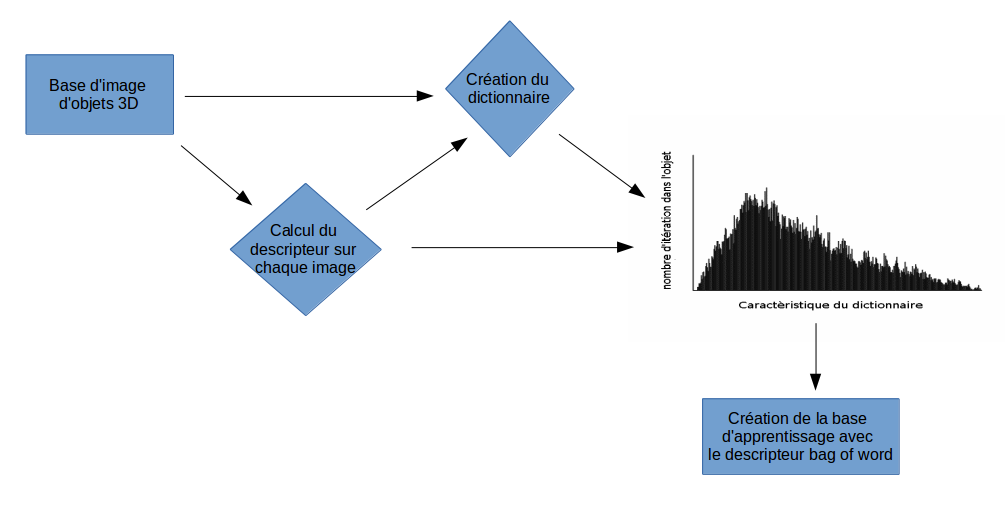
\includegraphics[height=8cm]{image/schemaBase.png}
    \caption{Schéma de la création de la base d'apprentissage}
  \end{center}
\end{figure}

%TODO parler des résultats de la reconnaissance

\subsection{Interface utilisateur}
L'interface utilisateur comprend deux fenêtres. La première comporte une vue avec le nuage de points récupéré à partir de la Kinect
et un ensemble d'options. Parmi ces options, nous avons la navigation dans le nuage de points et le choix de la technique de 
sélection. La première sélection est une simple sélection rectangulaire où l'ensemble des données à l'intérieur d'un rectangle formé
par deux points est sélectionné. La seconde est une sorte de pinceau sélectionnant les données en dessous de la souris, ainsi que celles dans 
un voisinage prédéfini autour de celle-ci. Lorsque l'utilisateur a sélectionné un objet et que l'application l'a reconnu, un nombre \textit{n} de cases 
avec des objets apparaît. Les objets dans ces cases sont les mêmes que l'objet sélectionné. Lorsque l'utilisateur clique sur l'une 
de ces cases, l'objets correspondant est ajouté dans la seconde fenêtre.
La seconde fenêtre contient l'environnement final dans lequel il y a déjà une piéce modèlisée avec des objets 3D. L'objet sélectionné est 
ajouté dans cette environnement.

\begin{figure}[!h]
  \begin{center}
    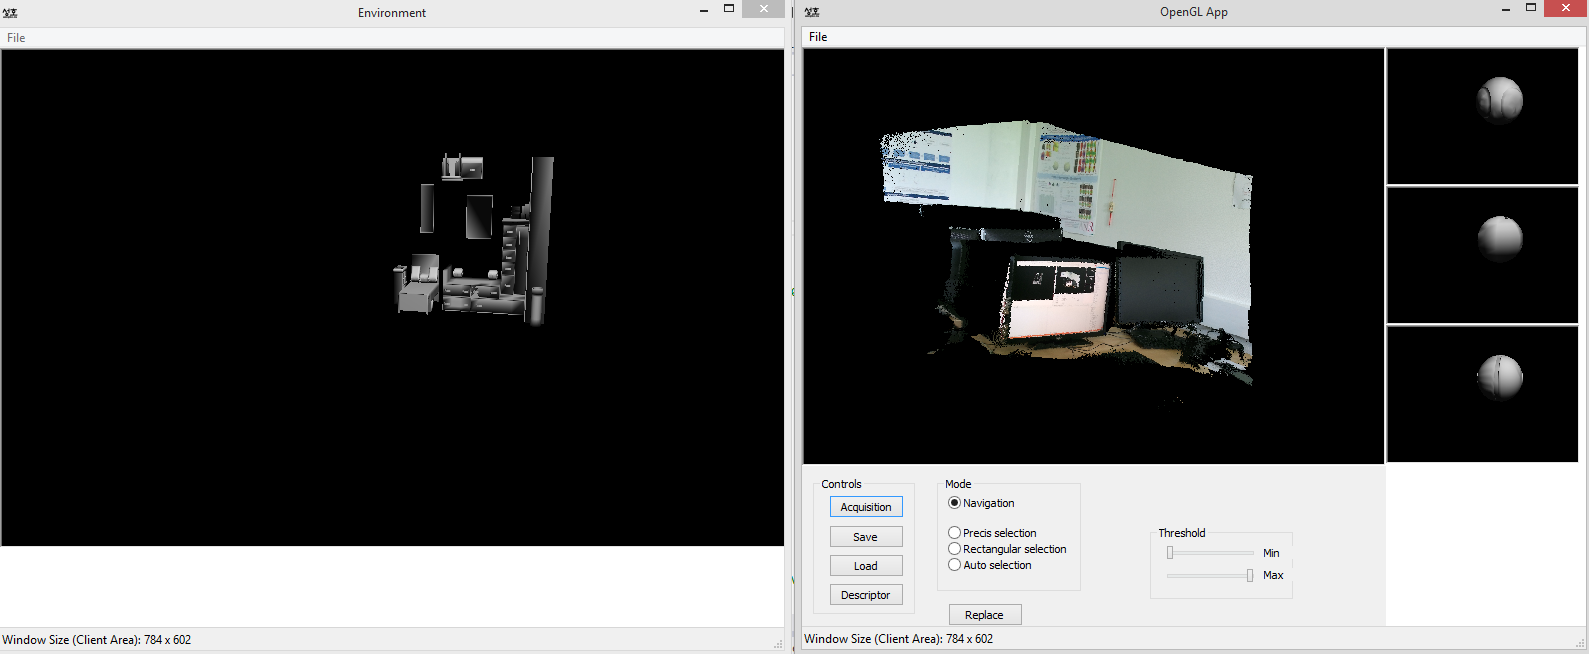
\includegraphics[height=7cm]{image/appliObjet.PNG}
    \caption{Interface de la seconde application}
  \end{center}
\end{figure}

\subsection{Travaux futures et applications}


%%%%%%%%%%%%%%%%%%%%%%%%%%%%%%%%%%%%%%%%%%%%%%%%%%%%%%%%%%%%%%%%%%%%%%%%%%%%%%%%%%%%%%%%%%%%%%%%%%%%%%%%%%%%%%%%%%%%%%%%%%%
%\section{Evaluation des méthodes}
%TODO aucune méthode d'évaluation déterminé

%%%%%%%%%%%%%%%%%%%%%%%%%%%%%%%%%%%%%%%%%%%%%%%%%%%%%%%%%%%%%%%%%%%%%%%%%%%%%%%%%%%%%%%%%%%%%%%%%%%%%%%%%%%%%%%%%%%%%%%%%%%
\section{Conclusion}
Durant ce stage j'ai réalisé deux projets permettant de réaliser la segmentation d'objet complexe comme le corps
humain et d'une scène intérieur à partir d'image 3D provenant d'une caméra Kinect. L'objectif était de créer
des interfaces permettant de faciliter la tâche des professions artistiques en leur permettant d'utiliser 
des objets du monde réelle dans un environement virtuel. Dans la première application sur le corps humain,
nous avons cherché à récupérer les informations du corps de la personne en face de la caméra et de segmenter
ces informations. Les informations ainsi segmenté pouvait ensuite être remplacé par l'utilisateur afin de 
pouvoir mettre des éléments virtuel sur un corps venant du monde réel. Pour réalisé ce projet nous avons 
utilisé les algorithme fournis dans le SDK de la Kinect pour filtrer les données. Etant donné la différence
des données entre le nuage de points que nous récupérons de notre caméra et les modèle 3D que nous utilisons,
nous avons privilégié une méthode basé sur l'utilisation des caractèristiques de la boîte englobante pour
déterminer la position et l'orientation du nuage de points de la partie du corps à remplacer. Ces informations
nous permettent ainsi de transformer le modèle 3D pour que celui-ci soit exactement à la même position que
l'ancien nuage de points. Le problème de notre méthode est q'une boîte englobante est une représentation 
beaucoup général pour une forme et donc l'orientation du nouveau modèle possède souvent une erreur de 90\degre
sur l'un des trois axes de la boîte. Pour l'application final, nous avons pensé proposer à l'utilisateur de 
corriger ce problème en sélectionnant l'axes qui fait défaut et l'application de chargerait d'appliquer la
bonne rotation au modèle.\\

La seconde applications avait pour but de prendre un environnement virtuelle dans laquel nous pouvons rajouté des éléments 
du monde réel. Ces objets du monde réel vienne du scanne d'une pièce via la caméra Kinect. La encore le processus nécessitait 
la segmentation des données afin de détecter les objets présents dans la pièce réel. La segmentation est réalisé 
par l'utilisateur qui doit sélectionné l'objet qu'il veut importer dans le monde virtuelle. Pour que l'application
reconnaisse l'objet qui a été sélectionné, nous avons utilisé un algorithme d'apprentissage automatique, les SVM,
avec le descripteur du sac de mot formé à partir du descripteur FPFH.\\
%TODO ajout des résultat de la méthode.

Lors de ce stage j'ai eu l'occasion de perfectionner les connaissances que j'avais acquise lors de mon master.
Les notions que j'avais vu de reconnaissance d'objet m'ont évidemment était très utile durant le stage, mais 
beaucoup de concept n'ont pas été approfondie durant les cours par manque de temps. J'ai pu approdonfir mes 
connaissance concernant les algorithmes d'apprentissage automatique et j'ai pu voir le fonctionnement de plusieurs
descripteur.\\ 

Le plus compliqué lors de ce stage a été de comprendre et tester des méthodes proposé dans des publications scientifique.
Certaine méthode n'était pas très complexe est facile à tester, mais de nombreuses publications se reposaient sur des connaissances
mathématique qui n'ont pas été vu durant mon cursus scolaire. Mais cette expérience m'a appris à réaliser un état de l'art des 
solutions existantes sur un sujet très spécifique et à tester les méthodes proposé dans la littérature. Ma seconde difficulté
lors de ce stage est que le sujet était assez vaste et qu'il ne fallait se perdre dans des méthodes qui s'éloigné du sujet.
Cela m'a appris à rester concentrer sur l'objectif principale en prévoyant et en organisant les étapes du projet.\\ 

Ce stage m'a fait redécouvrir l'environnement de la recherche dans lequel je souhaitais partir. Bien que j'ai réussi à surmonter
les difficultées que j'ai rencontré durant ce stage, il m'a permis de voir que l'environnement ne me convenait pas. La partie 
état de l'art, bien que très intéressante, a été assez difficile à réaliser. De plus, j'ai ressenti une certaine frustration
concernant les résultats du projet. J'ai passé énormément de temps à tester des méthodes difficile à implémenter et j'obtenais
que rarement des résultats intéressant pour mon projet. Ce stage m'a permis de comprendre que le monde de l'entreprise me
convenait mieux.

%resultat des deux projets
%ce que j'ai utilisé
%ce que j'ai appris
%comment me servir de mon stage pour après mes études

\newpage
\bibliographystyle{ieeetr} % or try abbrvnat or unsrtnat or plainnat
\bibliography{biblio}

\end{document}
